\section{Trees and tree-to-tree functions}
\label{sec:trees-transductions}
 In this section, we describe the trees and tree-to-tree functions that are discussed in this paper. 
%  The  trees are rooted, node labelled, ranked (the label of a node determines the number of children) and sibling ordered (there is a first child, second child, etc.). 
A \emph{ranked set} is a set where each element has an associated \emph{arity} in $\set{0,1,2,\ldots}$. We adopt the convention that ranked sets are red, e.g.~$\rSigma$ or $\rGamma$, and other objects (elements of ranked sets, or unranked sets) are black.  We use ranked sets as building blocks for trees. The following picture describes the notion of trees that we use and some terminology:
\mypic{1}

% When talking about elements of a ranked set, we mean elements of the underlying set.   For a ranked set $A$ and a finite set of variables $X \subseteq \varnames$, we write $\slice A X$ for the elements of $A$ that have arity $X$. 

We use standard tree terminology, such as ancestor, descendant, child, parent. We write $\trees \rSigma$ for the (unranked) set of trees over a ranked set $\rSigma$. This paper is about \emph{tree-to-tree functions}, which are functions of the type \begin{align*}
f : \trees \rSigma \to \trees \rGamma.
\end{align*}
%We also discuss tree languages, i.e.~sets of trees. 
%A tree language can be viewed as the special case of a tree-to-tree function, where the output alphabet $\Gamma$ contains only two letters ``yes'' and ``no'' of arity zero. Later on, we will also discuss terms, which are trees with variables. 

  
\subsection{First-order logic and transductions}
To define tree-to-tree functions and tree languages, we use  logic, mainly first-order logic and monadic second-order logic \mso. The basic idea is to view a tree as a model, and to use logic to describe properties and transformations of such models.

A \emph{vocabulary} is defined to be a set of relation names, each one with associated arity.  We do not use function symbols in this paper. A  vocabulary can be formalised as a ranked set, which is why we use red letters like $\ranked \sigma, \ranked \tau$ for  vocabularies. 

\begin{definition}[Tree as a model]\label{def:tree-model}
   For a tree $t$  over a ranked alphabet $\rSigma$, its \emph{associated model} 
%    $\underline t$
    is defined as follows. The  universe is the nodes of the tree, and it is equipped with the following relations:
   $$\begin{array}{lcll}
   x<y &  &   \text{$x$ is an ancestor of $y$} & \text{arity 2}\\
   \mathrm{child}_i(x) &  & \text{$x$ is an $i$-th child ($i\in \set{1,2,\ldots}$)} & \text{arity 1} \\
   a(x) &  &   \text{$x$ has label $a$ ($a \in \rSigma$)} & \text{arity 1}
   \end{array}$$
    \end{definition}

The $i$-th child predicates are only needed for $i$ up to the maximal arity of letters in the ranked alphabet, and hence the vocabulary in the above definition is finite. We refer to this vocabulary as \emph{the vocabulary of trees over $\rSigma$}.
 A sentence of first-order logic (or  \mso)  over this vocabulary   describes a tree language, namely the set of trees whose associated models satisfy the sentence.  For example, the sentence 
 \begin{align*}
 \forall x \ a(x) \Rightarrow \exists y \ x < y \land b(x)
 \end{align*} 
 is true in (the models associated to)  trees $t$ where every node with label $a$ has a descendant with label $b$. For more background about defining properties of trees using logic, see the survey of Thomas~\cite{thomas1997languages}.
 
 The regular tree languages are exactly those that can be defined in \mso, which was proved by Doner~\cite[Corollary 3.11]{Doner70}, and also Thatcher and Wright~\cite[p.~74]{thatcherGeneralizedFiniteAutomata1968}. The tree languages definable in first-order logic are a proper subset  of those definable in \mso, and it is an open problem whether or not one can decide if a regular tree language can be defined in first-order logic~\cite[Section 3]{bojanczyk2015automata}. This is in contrast to the case of words, where the decidable characterisation of  first-order logic by Sch\"utzenberger-McNaughton-Papert~\cite[Theorem 10.5]{McNaughtonPapert71} is  a cornerstone of algebraic language theory.
 
 \paragraph*{Tree-to-tree functions.}
 Apart from defining tree languages, first-order logic can also be used  to define transformations on  models. In the context of this paper, we are interested in first-order transductions, defined below.  Roughly speaking, a first-order transduction uses first-order logic to define a new tree structure on the input tree.

%  Define an \emph{$n$-ary  first-order query for trees over  $\rSigma$} to be a first-order formula $\varphi(x)$ with one free variable, which uses the  vocabulary of models associated to  trees over $\rSigma$, as per Definition~\ref{def:tree-model}. Given a tree over $\rSigma$, a unary  query selects a subset of nodes. An example of a unary query is ``$x$ has at least four ancestors''. 


\begin{definition}[First-order tree-to-tree transduction] \label{def:fo-transduction} A tree-to-tree function is called a  \emph{first-order transduction} if it can be obtained  by composing any number of operations\footnote{There is a normal form of first-order transductions, namely at most two phases are needed: first  item 1 and item 2. We do not need the normal form, so we do not prove it, but it can be shown similarly to~\cite[Section 7.1.5]{courcelle1991}. } of the following two kinds:
\begin{enumerate}
    \item \emph{Copying.} Let  $k \in \set{1,2,\ldots}$. Define  $k$-copying to be the operation which inputs a tree and outputs a tree where every node is preceded by a chain of $k-1$ unary nodes with a fresh label $\blueball$, as in the following picture:
    \mypic{94}
    After $k$-copying, the number of nodes grows $k$ times.
    \item \emph{Non-copying first-order transductions.} This is a tree-to-tree function which uses first-order logic to define a new tree structure over the nodes of the input tree. The syntax of such a transduction is given by:
     \begin{enumerate} 
        \item  \emph{Input and output alphabets} $\rSigma$ and $\rGamma$, which are finite ranked sets. We use the name \emph{input vocabulary} for the vocabulary of trees over the input alphabet $\rSigma$, likewise we define the \emph{output vocabulary}.
        % \item a \emph{copying constant} $k \in \set{1,2,\ldots}$;
        \item \label{it:universe-formula} A first-order formula over the input vocabulary, with one free variable, called the \emph{universe formula}.
        \item \label{it:tree-structure} For each relation of the output vocabulary, of arity $n$, a corresponding first-order formula  over the input vocabulary with $n$ free variables.
    \end{enumerate}
    The transduction inputs a tree over the input alphabet, and outputs a tree over the output alphabet where:
    \begin{itemize}
        \item the nodes  are those nodes of the input tree that satisfy the universe formula in item~\ref{it:universe-formula};
        \item the labels, descendant, and child relations are defined by the formulas in item~\ref{it:tree-structure}.
    \end{itemize}
    In order for the transduction to be well defined, the formulas in item~\ref{it:tree-structure} must be such that they produce a tree model for every input tree.
% \item \emph{First-order transduction.} A first-order transduction is any tree-to-tree function of the form: $k$-copying for some $k \in \set{1,2,\ldots}$, followed by a non-copying first-order transduction.
 \end{enumerate}
\end{definition}

If we allowed  monadic second-order logic \mso  in items~\ref{it:universe-formula} and~\ref {it:tree-structure} (the free variables of the formulas would  still be first-order variables ranging over tree nodes), then we would get the \mso tree-to-tree transductions of Bloem and Ensgelfriet~\cite[Section 3]{bloem_comparison_2000}. We will discuss these in  Section~\ref{sec:mso-trans}.


% By definition, first-order tree-to-tree transductions are closed under composition.   
We conclude this section with two examples of first-order tree-to-tree transductions. 
% A more elaborate example is in Appendix~\ref{sec:appendix-example-fo-transductions}.
% One can show that there is a normal form: in the first stage, one applied $k$-copying, and in the second stage one applies a non-copying first-order transduction. 
 %\footnote{   First-order transductions are  a special case of a first-order interpretations~\cite[p.~213]{hodges_model_1993}, which use tuples (instead of elements) in the input structure to describe elements in the output structure. As a result, first-order transductions have linear size increase, while first-order interpretations have polynomial size increase. First-order transductions are also a special case of \mso transductions, see~\cite[Section 7]{courcelle_graph_2012}, which use \mso logic instead of first-order logic, and which also allow a step where the input structure is nondeterministically coloured (and therefore the result is a binary relation on structures which is not necessarily functional).}

    
    

% \begin{definition}[First-order transduction]\label{def:fo-transduction}  A \emph{first-order transductions} is a function that inputs models and outputs models, which is obtained as a composition of two kinds of functions defined below, namely  $k$-copying (for some $k$) followed by a non-copying first-order transduction. 
% %\begin{enumerate}
%  %   \item 

%  1. \emph{Copying.} Fix some  relational vocabulary $\ranked \sigma$ and let $k \in \set{1,2,\ldots}$. Define $k$-copying to be the operation 
%     $$\begin{array}{lll}
%      \text{models over $\ranked \sigma$} & \to & 
%      \begin{array}{c}
%      \text{models over $\ranked \sigma$}\\ 
%      \text{extended with a $k$-ary relation $\mathrm{copy}$}
%      \end{array}
%     \end{array}$$
% which inputs a model $\mathbb A$, and outputs $k$ disjoint copies of $\mathbb A$, where the  $\mathrm{copy}$ relation is interpreted as the set of tuples $(a_1,\ldots,a_k)$ such that, for  some $a \in \mathbb A$, the first copy of $a$ is  $a_1$, the second copy of $a$ is $a_2$, etc. The $\mathrm{copy}$ relation  is not commutative, because we distinguish the copies.
% \smallskip

% 2.    \emph{Non-copying first-order transduction.} The syntax of a \emph{non-copying first-order transduction}  is given by:
% \begin{enumerate}
%     \item Input relational vocabulary $\ranked\sigma$ and output relational vocalbulary $\ranked{\gamma}$.
%     \item A first-order \emph{universe formula} $\varphi(x)$ over $\ranked{\sigma}$.
%     \item For every relation $R$ in vacubulary $\ranked{\gamma}$, a first-order  formula $\varphi_R(x_1,\ldots,x_{\arity R})$ over $\ranked{\sigma}$.
% \end{enumerate}
% The semantics of a non-copying first-order transduction is  a function
% \begin{align*}
%     \text{models over $\ranked\sigma$} \quad \to \quad \text{models over $\ranked\gamma$}
% \end{align*}
% defined as follows. If the input model is $\mathbb A$, then the output model is defined as follows: the universe is elements of $\mathbb A$ which satisfy the universe formula, and each relation $R$ is interpreted as those tuples that satisfy $\varphi_R$. 

% \smallskip
% % \end{enumerate}
% \end{definition}



% Every first-order  transduction has linear size increase, i.e.~if the input structure has a finite universe of size $n$, then the output structure has a universe of size at most $kn$, where $k$ is the number of copies used in the transduction. First-order transductions are easily seen to be closed under composition.

% \begin{definition}[First-order tree-to-tree transduction.]
%     A \emph{first-order tree-to-tree transduction} is any tree-to-tree  function which can be implemented by a first-order transduction, assuming that trees are modelled according to Definition~\ref{def:tree-model}. More formally, a first-order tree-to-tree transduction is any function $f$ which makes the following diagram commute
%     \begin{align*}
%         \xymatrix{
%             \trees \rSigma \ar[d]_{t \mapsto \underline t}\ar[r]^f & \trees \rGamma \ar[d]^{t \mapsto \underline t} \\
%             \set{\underline t : t \in \trees \rSigma} \ar[r]_g & \set{\underline t : t \in \trees \rGamma}.
%         } 
%     \end{align*}
% for some first-order transduction $g$.     
% \end{definition}




\begin{example}\label{ex:filter-first}
    Let the input and output alphabets be:\vspace{-15pt}
    \mypic{17}
    and consider the  function which removes the unary nodes:
\begin{center}
\includegraphics[scale=.35, page=19]{pics.pdf}
\end{center}
This is a non-copying first-order  transduction. The universe formula selects nodes which have non-unary labels. The descendant relation is inherited from the input tree. To define the child relation on the output tree, we need to use the descendant relation in the input tree. A node $x$  satisfies the unary  $i$-th child predicate   in the output tree if it satisfies the following first-order formula in the input tree:
\begin{align*}
    \exists y \ \child i (y) \land \underbrace{y \le x \land   \forall z\ (y \le z < x \Rightarrow \blueball(z))}_{\substack{\text{$y$ is the farthest ancestor that can be} \\ \text{reached from $x$ using only unary nodes}}}.
\end{align*}
% This example shows how the descendant relation is needed  that even tree-to-tree homomorphisms need the descendant relation (instead of a binary child relation, as used in)
%This function could not be implemented by a first-order transduction if we replaced the descendant relation by a binary parent-child relation.
\end{example}


\begin{example}\label{ex:pre-order-main} Define  \emph{pre-order} on nodes in a tree as follows:  $x$ is before  $y$ if either $x \le y$, or there exist nodes $x'$ and $y'$ such that $x' \le x$, $y' \le y$, and $x'$ is a sibling of $y'$ with a  smaller child number.  Consider  the tree-to-tree function which transforms a tree into a list of its nodes in pre-order traversal, as explained in the following picture:
    \mypic{112}
    This function is a first-order tree-to-tree transduction, 
    because the pre-order is first-order  definable. Unlike Example~\ref{ex:filter-first}, we need copying, because a node of arity $n$ in the input tree corresponds to $n+2$ nodes in the output tree.
\end{example}

